\documentclass{article}
\usepackage{latexsym}
\usepackage{amsmath}
\usepackage[a4paper]{geometry}
\usepackage{fullpage}
\usepackage{hyperref}
\usepackage{booktabs}
\usepackage{graphicx}
\usepackage{tikz}
\usepackage{xcolor}
\usepackage[export]{adjustbox}
\usepackage{comment}
\usepackage{subcaption}
\usepackage[style=iso]{datetime2}
\usepackage{cleveref}
%\usetikzlibrary{calc}
\usetikzlibrary{arrows,positioning} 
\tikzset{
    %Define style for course boxes
    courseboxv/.style={
           rectangle,
           draw=blue!50!black, very thick,
           fill=blue!10,
           minimum height=8cm,
           minimum width=4cm,
           text width=3.9cm,
           text centered,
           font=\bfseries\sffamily},
    courseboxh/.style={
           courseboxv,
           minimum height=4cm,
           minimum width=8cm,
           text width=7.9cm},
    courseboxhh/.style={
           courseboxh,
           minimum height=4cm,
           minimum width=16cm,
           text width=15.9cm}
}
\def\frameseparation{1.5cm}
\def\scalingfactor{.8}

\newcommand{\secref}[1]{Section~\ref{sec:#1}}
\newcommand{\secreff}[2]{Sections \ref{sec:#1} and \ref{sec:#2}}
\newcommand{\eqnref}[1]{Equation~\eqref{eq:#1}}
\newcommand{\eqnreff}[2]{Equations \eqref{eq:#1} and \eqref{eq:#2}}
\newcommand{\eqnrefff}[3]{Equations \eqref{eq:#1}, \eqref{eq:#2} and \eqref{eq:#3}}
\newcommand{\figref}[1]{Figure \ref{fig:#1}} 
\newcommand{\figreff}[2]{Figures \ref{fig:#1} and \ref{fig:#2}}
\newcommand{\figrefff}[3]{Figures \ref{fig:#1}, \ref{fig:#2} and \ref{fig:#3}}
\newcommand{\tabref}[1]{Table~\ref{tab:#1}}
\newcommand{\tabreff}[2]{Tables~\ref{tab:#1} and \ref{tab:#2}}
\newcommand{\tabrefff}[3]{Tables~\ref{tab:#1}, \ref{tab:#2} and \ref{tab:#3}}

\def\year{2024--2025}
\title{EITA65 Design of Systems for Digital Transformation\\\year}
%\title{EITA65 Digitalisering -- realisering och systemdesign med användarperspektiv\\\year}
\author{\huge Drone Simulation on Raspberry Pi\\Drone Project -- Part 1}
%\\Version \DTMnow}
%\date{}

\begin{document}
\newgeometry{left=2.5cm,right=2.5cm,bottom=1.5cm}% for placing course schematic lower on first page
\clearpage\maketitle
\thispagestyle{empty}% to remove page numbering on first page

\begin{itemize}
\item This project will be done individually, but you will work \textit{together} in groups of 3 or 4.
\item You will not get detailed step-by-step instructions. Figuring out how to reach the goal is part of the project. (being a collaborative doer)
\item The results of this project part will be used in the next, so document your work.
\end{itemize}

\vspace{.1cm}
\begin{center}
\begin{tabular}{l}
\toprule[1.5pt]
\parbox{0.8\linewidth}{
\vspace{.2cm}{\Large Learning goals:}
\begin{itemize}
\item Becoming familiar with web server development
  \begin{itemize}
  \item Understanding Flask framework.
  \item Understanding HTML and interaction between HTML object and your web server. 
  \item Understanding HTTP protocol and integration between client and server. 
  \item Familiarize yourself with the drone simulator package we will be using in the coming assignments.
  \end{itemize}
\item Practicing collaboration skills.
\end{itemize}}\\
\bottomrule[1.5pt]
\end{tabular}
\end{center}
\vfill
% \begin{center}
% \includegraphics[width=120mm]{rpi4_no_bg.png}
% \end{center}
%\vspace{1cm}

\begin{comment}
\begin{center}
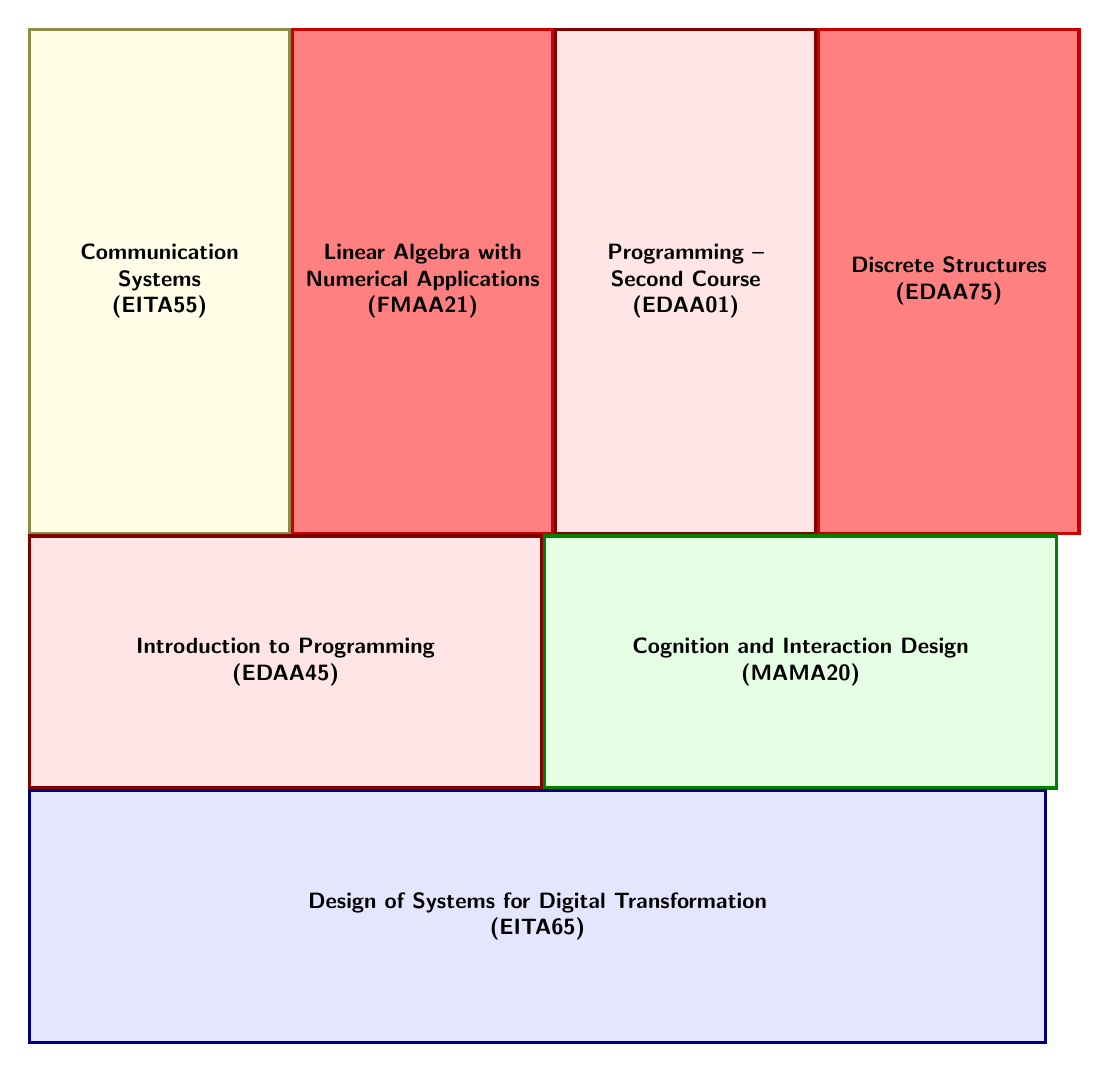
\begin{tikzpicture}[>=latex, node distance=0cm,scale=\scalingfactor,every node/.style={scale=\scalingfactor}]
\node[courseboxv, draw=yellow!50!black, fill=yellow!10] (EITA55) {Communication Systems\\(EITA55)};
\node[courseboxv, draw=red!80!black, fill=red!50, anchor=west] (FMAA21) at (EITA55.east){Linear Algebra with Numerical Applications\\(FMAA21)};
\node[courseboxv, draw=red!50!black, fill=red!10, anchor=west] (EDAA01) at (FMAA21.east){Programming -- Second Course\\(EDAA01)};
\node[courseboxv, draw=red!80!black, fill=red!50, anchor=west] (EDAA75) at (EDAA01.east){Discrete Structures\\(EDAA75)};
%\node[courseboxh, preaction={clip, postaction={fill=red!10, draw=red!50!black, line width=2mm}}, anchor=north west] (EDAA45) at (EITA55.south west){Introduction to Programming\\(EDAA45)};
\node[courseboxh, draw=red!50!black, fill=red!10, anchor=north west] (EDAA45) at (EITA55.south west){Introduction to Programming\\(EDAA45)};
%\node[courseboxh, draw=green!50!black, fill=green!10, anchor=west] (MAMA20) at (EDAA45.east){Cognition and Interaction Design\\(MAMA20)};
\node[courseboxh, draw=green!50!black, fill=green!10, right=of EDAA45] (MAMA20) {Cognition and Interaction Design\\(MAMA20)};
\node[courseboxhh, anchor=north west] (EITA65) at (EDAA45.south west){Design of Systems for Digital Transformation\\(EITA65)};
%\node[anchor=south east, inner sep=2pt, font=\bfseries\sffamily\scriptsize] at (EDA625.south east) {Helsingborg};
%\path[->,draw=black,dotted,thick] (EIT060.east) -- (EITF05.west);
%\path[->,draw=black,dotted,thick] (EIT060.south) -- (EITN50.north);
%\path[->,draw=black,dotted,thick] (EITF05.south) -- (EITN41.north);
%\draw[draw=blue!50!black, very thick] ($(EIT060.north west)+(-\frameseparation,\frameseparation)$) rectangle ($(EDA625.south east)+(\frameseparation,-\frameseparation)$);
\end{tikzpicture}
\end{center}
\end{comment}

\begin{center}
\includegraphics[width=90mm]{drone.pdf}
\end{center}

\restoregeometry
\newpage


\section{Introduction}
In this project part you will get more acquainted with a Flask web server, and work with a drone simulation hosted by the web server. In the simulation, you will get a map of Lund city on the web page, and control a 'drone', moving it on the map.

In the first part of this assignment, you will get functional code for the web server and the simulation. Please first take a look at the code you get, try it out and try to understand as much as you can. This instruction will also guide you to understanding it.\\

\noindent{\bf Note: }\parbox[t]{14cm}{{You will get some questions marked in red in this instruction. You need to write down the answers and show to the TAs after you finish the assignment.}}\\

\begin{comment}
You can run this code on your own computer, lab computer or on your Raspberry Pi (If you are using MAC OS and get problem with \texttt{}pip3, Read the Hint). But make sure your device is connected to the Internet when you are running the web server. In the second part, your Raspberry Pi will be needed for the implementation. You will get to modify the provided code, and control the 'drone' on the map by using the joystick on the Pi Sense HAT.
\end{comment}

\section{Clone the code and try it out}
Get the code from this {\color{blue}\href{https://github.com/rogerhenriksson/InfoCom-Drone-1-Intro}{GitHub repository}} ({\small \texttt{https://github.com/rogerhenriksson/InfoCom-Drone-1-Intro}}). Clone or download it to your Raspberry Pi. It is highly recommended that you fork this repo to your own account, and clone the forked one. Alternatively you can create a new Git repo and put the downloaded files in it. In this way, when you make changes in the code, you can commit the changes, and push your commits to your repository. So if your Raspberry Pi crashes or if you need to switch device, you always have your up-to-date code in your repository.

You can follow the instructions in the \texttt{README.md} file to deploy the web server and run 'controller' of the 'drone' with your keyboard. Now let's glance at the code and try to understand how this simulation is deployed.

\begin{figure}[h!]
    \centering
    \includegraphics[trim=200 100 200 200,clip, width=100mm]{map.png}
    \caption{Map of Lund}
    \label{fig:map}
\end{figure}

\subsection{The Map}
When you successfully deployed the web server, open the website in your web browser, you can see a map of Lund that looks like \Cref{fig:map} hosted by the website. It is a map of Lund composed by edges and vertices (or nodes). The geographic coordinates of all the components in the map are from OpenStreetMap (OSM) \cite{OSM}. The edges represent the actual streets in Lund, and nodes are the intersections of the streets.


The red dots (a circle element in CSS) on the map represents the drone location, and the coordinates of the drone are also displayed on the web page.

The elements of the web page can be seen in the \texttt{/webserver/templates/index.html} file. JavaScript was used to create all the elements and you don't need to edit the JavaScript-section in your tasks of this assignment, but you can try to modify the HTML file a bit and add CSS if you want to change the layout or have a better design of the website.

The map image is in SVG format - it is a vector image format for two-dimensional graphics. This image is stored in \texttt{/webserver/static/images/}. If you open this image in your programming IDE, you can see it is formed with many vectors with coordinates. Therefore, every point in this SVG image has coordinates. However, the SVG image and OMS have different coordinate systems, that means the same location gets different coordinates from OSM and from the SVG image. The relation between the two coordinate systems are shown in \Cref{fig:OSMtoSVG}.  In this case, when you get a pair of location coordinates (longitude, latitude) from OSM, you will need to convert it to (x, y) in the SVG coordinate system. This is done by the \texttt{translate(coords\_osm)} function given in \texttt{/webserver/build.py}. In this assignment, you only work with OSM coordinate system to move the drone, the function will translate it to SVG coordinates before passing the location data to the HTML file and showing it on the map.\\

\noindent{\bf Question 1: }\parbox[t]{14cm}{\textcolor{red}{The drone's location is initialized on the map when you open the browser, find out the initial coordinate in (longitude, latitude) and in SVG (x,y).}}


\begin{figure}[h!]
    \centering
    \includegraphics[width=120mm]{coords_sys.png}
    \caption{Relationship between OSM and SVG coordinate systems}
    \label{fig:OSMtoSVG}
\end{figure}

\subsection{The web server}
In the Python script of the web server \texttt{webserver/build.py}, you can also see three functions with decorators (Python decorators are indicated by @ symbol before each function, see \cite{deco} for what a decorator is). Two functions with \texttt{@app.route()} means that they can be called by HTTP requests. The \texttt{@app.route('/')} is the default function that will be called when you type the URL \url{http://127.0.0.1:5000} in your browser, and you can see it renders the \texttt{index.html} file, which contains all the objects of your webpage. 

You can also see another route \texttt{/drone}, which will call the \texttt{drone()} function. Add \texttt{/drone} to the link on your browser to try to access it.\\

\noindent{\bf Question 2: }\parbox[t]{14cm}{\textcolor{red}{Explain what message you get from the browser and why you get the message.}}\\


Another decorator is \texttt{@socket.on()} used by \texttt{get\_location()}. If you look at the terminal that runs the web server, you can see it keeps printing out something like \texttt{"GET /socket.io/?...HTTP/1.1" 200} in the terminal, this is because a HTTP client keeps making requests that calls the \texttt{get\_location()} function.\\

\noindent{\bf Question 3: }\parbox[t]{14cm}{\textcolor{red}{Please go through all the files that are provided in the \texttt{/webserver} directory and find out where the client that makes the requests is, and why it makes the requests.}}


\subsection{Drone controller}
Now it's time to look at the script \texttt{/pi/pi\_controller.py}. When you run this script, you can type on arrows keys or 'wasd' keys on your keyboard, and move the drone on the map displayed on your website.

There are two parts in the script: \texttt{if \_\_name\_\_ == "\_\_main\_\_"} indicates that it is the main function of this script, and that is where you start when you run this Python script; \texttt{get\_direction()} is called by the main function. It reads the keyboard and returns the movement in longitude and latitude represented by the key to the main function. The main function makes a request with the movement values to the web server that calls the \texttt{map()} function. Read the code in the script and the \texttt{map()} function in \texttt{/webserver/build.py}.\\

\noindent{\bf Question 4: }\parbox[t]{14cm}{\textcolor{red}{Find out the distance a drone is moved in longitude and latitude by each key you pressed.}}





\section{Write your own controller}
In this assignment, you will need to run the web server and the controller on your Raspberry Pi. Your task is to modify the controller in \texttt{/pi/pi\_controller.py}. In the provided script, you used the keyboard to move the drone. Now you need to replace the \texttt{get\_direction()} with your own, so that the drone is moved by the joystick on your Raspberry Pi, similarly to how it is moved by the arrow keys in the original script. {\textcolor{red}{You need to show the TAs your completed task when you have finish it.}


\begin{comment}\section{Hint for MAC OS}
\label{sec:mac}
If you run the web server on MAC OS, you may get problems with \texttt{pip3}. MAC has Python3 installed by default in the system, but depending on your OS version it might not have pip3. There are several ways to install pip3 if you google "How to install pip3 on MAC OS". The easiest one you find may be \texttt{brew install python3}. The command \texttt{brew} is the most popular package manager on MAC OS (like \texttt{apt} in Debian), but when you install with \texttt{brew}, you install the whole python3 again in your system, but in a different path. This path is not in your default system PATH, so your computer will not understand that you wants to use the newly installed python3. Therefore, you need to add the new path to your system PATH in \texttt{~/.bash\_profile} or \texttt{~/.zshrc}, source the changed file and you should be able to use the newly installed \texttt{python3} and \texttt{pip3}.
\end{comment}

% {\bf Hint 1: }\parbox[t]{14cm}{Check for updates to this document. Instructions may have been clarified in a more recent version. You can find the version number of the document on the very first page. The version number is the compile-date of the document in ISO-format~\cite{iso-date-time}.}\\
% {\bf Hint 2: }\parbox[t]{14cm}{To avoid rewriting many commands, you can use the keys \texttt{arrow up} and \texttt{arrow down} to go back and forth between the commands that you just wrote.}\\
% {\bf Hint 3: }\parbox[t]{14cm}{To paste commands into the terminal you can use \texttt{Ctrl + Shift + V}}\\
% {\bf Hint 4: }\parbox[t]{14cm}{tab in instructions}\\
% {\bf Hint 5: }\parbox[t]{14cm}{To avoid rewriting many commands, it can be a good idea to write all steps in a batch-file or shell script. Then you can also reuse the batch file for the second project.}
\vspace{1cm}
\begin{center}
\huge Good luck!
\end{center}

\begin{thebibliography}{10}
\bibliographystyle{plain}

\bibitem{OSM} OpenStreetMap, \url{https://www.openstreetmap.org/#map=14/55.7059/13.2005}, last accessed on 2021-11-08.

\bibitem{deco} Python decorator, \url{https://python-3-patterns-idioms-test.readthedocs.io/en/latest/PythonDecorators.html}, last accessed on 2021-11-08.


\end{thebibliography}

\end{document}
